% Features & App Design
% • List and description of the individual features within the application
% • Any storyboards illustrating the core features of the application (MISSING)
% • Description of the storyboards
% • UI Prototypes of the core features of the application
% • Description of the features illustrated by the prototypes

\chapter{Design}\label{ch:design}

\section{Storyboard}

\begin{figure}[h]
       \centering
       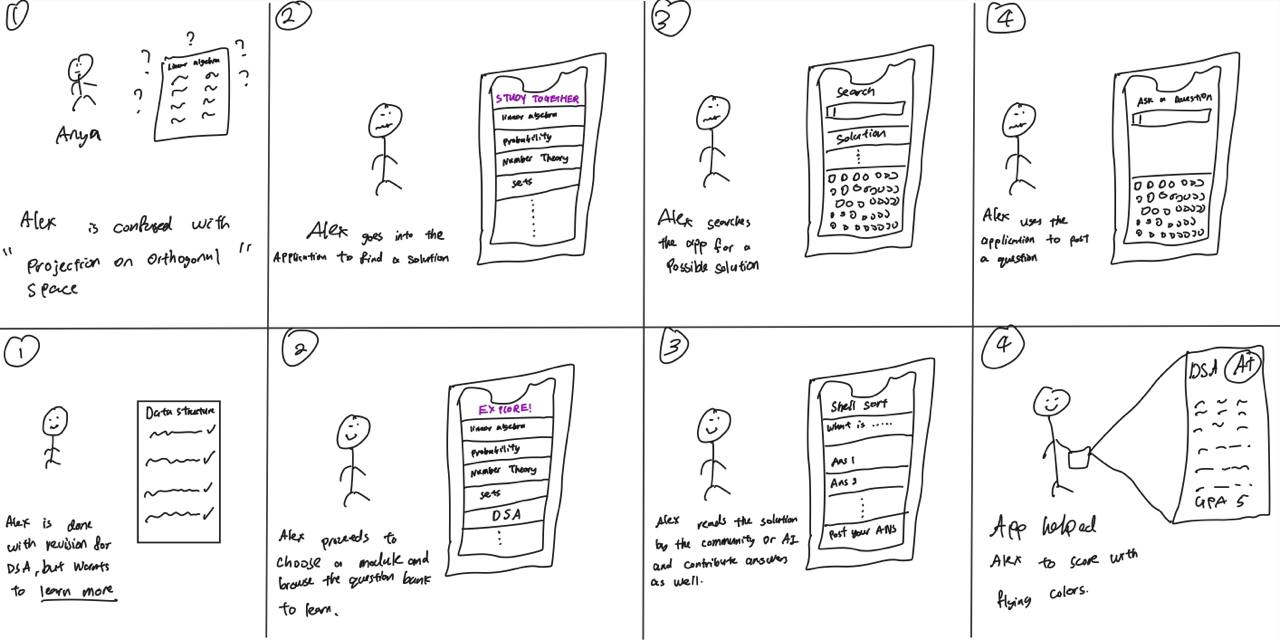
\includegraphics[width=\textwidth]{Figures/storyboard.jpg}
       \caption{Storyboard of Use Cases}
       \label{storyboard}
\end{figure}

The storyboard above illustrates two scenarios featuring our persona, Alex, and his journey through higher education.

In the first scenario (top), Alex encounters confusion while studying Linear Algebra, specifically struggling with the concept of projection on orthogonal space. To seek assistance, he utilizes our "Study Together" application to search for a solution. If no similar questions are found, Alex proceeds to post his query.

In the subsequent scenario, Alex has completed his revision but desires further understanding of a particular topic, specifically Data Structures and Algorithms. He navigates to the application's explore section or conducts a targeted search for the topic of interest, focusing on "Shell Sort". The final image portrays Alex achieving academic success after leveraging our application's peer-to-peer learning platform.

This storyboard effectively captures Alex's educational journey, highlighting the pivotal role our application plays in facilitating learning and knowledge exchange.


\section{Features}

\subsection{User Authentication and Personalization}

The application incorporates robust user authentication mechanisms to ensure secure access to personalized features. Upon registration, users can create profiles, customize preferences, and follow or unfollow other users based on their interests. This personalized experience enhances user engagement and fosters a sense of community within the platform.

\subsection{Post Question/Answers}

Users can seamlessly post questions or provide answers within the application's intuitive interface. This feature facilitates knowledge sharing and collaborative learning, empowering users to seek assistance or contribute insights on various topics. The ability to interact through questions and answers enriches the learning experience and promotes peer-to-peer support among users.

\subsection{AI Generated Answers}

To enhance the efficiency of knowledge exchange, the application integrates AI-generated answers. Leveraging advanced algorithms, users can receive accurate and insightful responses to their queries, augmenting the platform's capabilities for providing valuable assistance and guidance on diverse subjects. This feature also provides users with a sample answer they can refer to if their question remains unanswered, saving them time and effort from manually seeking answers from other AI assistant tools, such as ChatGPT.

\subsection{Wolfram|Alpha Service Generated Answers}

Our application offers a seamless solution for answering math questions by integrating a Wolfram|Alpha retrofit API service. This service serves as a backup for the Gemini AI API, particularly for math queries that the AI may struggle with. By leveraging Wolfram|Alpha's expertise in mathematical computations, users can receive accurate answers to their math-related inquiries, ensuring a comprehensive and reliable knowledge exchange experience. This integration enhances the platform's capabilities, providing users with a wider range of answers and ensuring that they can always find the information they need, regardless of the complexity of the question.

\subsection{OCR Scanning for Easy Question Creation}

The OCR scanning feature simplifies the process of creating questions by allowing users to scan printed text. This innovative functionality converts scanned text into digital format, enabling users to effortlessly generate questions and contribute to the platform's knowledge base. Images can be cropped within the app and the text output can be edited before inserting to the textfield.

\subsection{Explore Section}

The Explore section provides users with curated content, including trending questions, popular tags, and recommended users to follow. This feature enhances user engagement by showcasing relevant and interesting content, facilitating exploration and discovery within the platform. By presenting diverse topics and users, the Explore section enriches the user experience and encourages interaction among community members.

\subsection{Home Screen Feed}

The Home Screen Feed offers users a personalized view of content from the users they follow. By aggregating posts and updates from followed users, this feature enables users to stay informed and engaged with the latest discussions and developments within their network. The Home Screen Feed fosters a sense of connection and community by presenting tailored content based on individual preferences and interests.

\subsection{Chat Interface}

The Chat Interface facilitates private communication between users, offering a platform for exchanging messages and queries. Users can engage in confidential conversations, asking questions or sharing information without concerns about their messages being shared with others. This feature ensures discretion, empowering users to communicate freely with one another. 

\subsection{Pastel Color Schemes}

The application's design incorporates pastel color schemes inspired by Catppuccin, creating a visually appealing and cohesive user interface. Soft hues and gentle tones contribute to a calming and inviting aesthetic, enhancing the overall user experience. The use of pastel colors adds warmth and personality to the application, creating a welcoming environment for users to engage and interact.

\subsection{Notification Feed}

The notification feed in "Study Together" is meticulously designed to showcase only the daily new posts, establishing a distinct experience from the home screen feed. While the home screen aggregates all updates and posts from followed users, the notification feed is refined to present only the most recent daily posts. This delineation ensures a clutter-free and streamlined view, enabling users to efficiently peruse all new content at a single glance each day. This approach not only simplifies content discovery but also enhances the app’s usability by minimizing information overload and optimizing the user’s daily engagement with fresh material.

Additionally, such a design choice may encourage regular app engagement, as users can develop a habit of checking the daily notification feed for updates without having to navigate through already viewed content. If desired, future iterations of the notification system could include features such as personalized summaries or highlights of the most interacted-with content, offering an even more tailored and efficient user experience.

%%%%%%%%%%%%%%%%%%%%%%%%%%%%%%%%
% UI Prototypes 
%%%%%%%%%%%%%%%%%%%%%%%%%%%%%%%%
\import{Sections/}{UI_Prototypes}
